\section{问题二：同核驻留与跨核同步下的调度}
\subsection{场景 B 的模型扩展}
问题二仍选择 $(\pi,m,\sigma)$，但场景 B 不再把每个子图独立清空为一个 Task：映射到同一核心的全部子图组成该核的 Task，核内合法顺序决定缓存复用与张量生命周期。对于同一张量，若生产和消费能够在同核满足依赖，则中间结果可以驻留；跨核消费必须按实际生产核与消费核构造搬运，并在源 \texttt{COPY\_OUT} 完成后经过 $500$ cycles 才能释放目标 \texttt{COPY\_IN}。对于跨核数据事件 $e$，有
\begin{equation}\label{eq:q2-release}
a_e^{\mathrm{in}}\ \ge\ f_e^{\mathrm{out}}+500.
\end{equation}
这里的前驱是具体搬运事件，而非“源子图全部运行完”的粗粒度时刻。对多消费者共享张量，外部输入按消费核心而非每个算子独立读取；跨核中间张量按实际源核—目标核关系生成，避免把每条逻辑边简单等同一次物理 COPY。

合法集合 $\mathcal P_B(k)$ 除保留覆盖、子图商图和核上顺序的无环性外，还要求由官方核内展开得到的物理实例满足 L1/UB 在每个时刻的容量约束。四条 Pipe 各自串行，但不同 Pipe 在依赖允许时可重叠；同一 DDR 池服务所有在途外存搬运。张量能否驻留依赖实际产生、消费和溢出时刻，不能只按静态张量大小之和判断。令 $\mathcal E_B$ 表示题目的事件模拟，问题二的目标为
\begin{equation}\label{eq:q2-objective}
\min_{p\in\mathcal P_B(k)}
\operatorname{lex}\left(T_i^B(p),D_i(p)\right),\qquad
T_i^B(p)=\mathcal E_B(G_i,p;k).
\end{equation}
这仍是依赖官方事件过程的组合优化模型，不把启发式估价器当作精确求解的线性目标。与问题一相比，映射会同时改变通信、驻留、释放和并行，所以切图后固定映射、或仅按分组时长排序，均可能错过有效方案。处理器互连与片上存储的耦合也是相关体系结构研究关注的问题\cite{t10}；本题仍以给定的缓存及 COPY 语义为准，不移植其他硬件的通信规则。

\subsection{从独立 Task 到每核联合 Task}
场景 B 保留同一个划分 $\pi$、核心映射 $m$ 和核上顺序 $\sigma$ 决策，但改变了这些决策的物理含义。对每个核心 $c$，把映射到 $c$ 的全部子图按 $\sigma_c$ 展开到一个 Task 的内部：子图之间仍有次序，然而私有 L1/UB 状态在这段次序中连续存在。若生产与最后消费同在 $c$，中间张量可在容量允许时直接驻留；外层切出两个子图并不自动产生一次 DDR 往返。相反，两个核心之间的依赖须经源端写出、目标端读入与同步释放。由此，场景 A 的“每跨一个子图边界就增加传输”在 B 中不再成立，决策的风险从 Task 边数转向跨\emph{核心}的逻辑张量集合与同核生命周期长度。

记 $c_p(x)$ 为内部张量 $x$ 的生产核心，$\mathcal C(x;p)=\{m(\pi(v)):v\in C(x)\}$ 为消费核心的去重集合。目标核心数
\begin{equation}\label{eq:q2-destination-count}
n_{\rm remote}(x;p)=
\bigl|\mathcal C(x;p)\setminus\{c_p(x)\}\bigr|
\end{equation}
给出跨核心\emph{目的地}的数目，而不是跨核算子边条数。若同一核心有三个消费算子，集合里仍只出现一次。对于原始外部输入，不存在内部生产核心；其各消费核心可共享一次该核心的加载机会。这个去重关系用于静态候选估价，但是否产生源端一次或多次 COPY、原图已经有多少基础 COPY、是否因容量溢出再读，均由官方 Task 构造及核内展开确定。因此问题二沿用
\begin{equation}\label{eq:q2-added-exact}
D^B(p)=B_{\rm all}^{B}(p)-B_{\rm orig},
\end{equation}
作为可交付的额外搬运定义；不直接把 $b_x n_{\rm remote}(x;p)$ 宣称为总额外字节。对按边计费的朴素代理，令 $\mathcal E_x^{\rm remote}$ 为张量 $x$ 的跨核消费者边集合，则目标核心去重的\emph{读入字节代理}满足
\begin{equation}\label{eq:q2-dedup-inequality}
b_x\,n_{\rm remote}(x;p)
\ \le\ b_x\,|\mathcal E_x^{\rm remote}|.
\end{equation}
不等号可严格成立，说明朴素边权和可能高估共享消费者的通信，从而错误惩罚本应考虑的划分。

\subsection{跨核释放与事件路径}
对一个源核心 $a$ 到目标核心 $b$ 的张量传递，设 $e^{\rm out}$ 为源端对应 \texttt{COPY\_OUT}，$e^{\rm in}$ 为目标端 \texttt{COPY\_IN}。在场景 B，后者的发射条件是
\begin{equation}\label{eq:q2-sync-expanded}
s_{e^{\rm in}}\ge f_{e^{\rm out}}+\delta_B,
\qquad \delta_B=500\ {\rm cycles}.
\end{equation}
等待从\emph{实际写出完成}开始计，不是从源子图的名义结束开始计。若源核还有与这份张量无关的矩阵计算，这段计算可能在写出完成后继续；目标核只需等待它自身需要的 COPY 就绪，而不是盲等源核整个 Task 完成。一个目标操作若依赖多个数据来源，其就绪时刻取相关发射与完成约束的最大值。把多条前驱的 $500$ 周期全部相加，会夸大并行等待；把所有源 Task 一起拉长 $500$，则会错误阻塞无关 Pipe。表\ref{tab:scenario}所示三个场景在此处产生的差别，必须在事件层而非仅在子图时长层表达。

场景 B 的完整事件依赖包括：原算子数据边、各 Pipe 的顺序边、跨核 COPY 写出到读入的释放边，以及官方核内启发式插入的内存复用和换入换出边。若把所有源到汇路径记为 $\Gamma_B(p)$，则在真实事件服务时长确定后仍可使用式\eqref{eq:realized-critical-path}解释总时间；但搜索前无法仅由子图大小求得这些路径。特别地，跨核释放 $\delta_B$ 可以与另一核心的计算并行，只有位于决定最终输出的路径时才直接增加 Makespan。

\subsection{真实物理驻留与容量约束}
令 $\mathcal R_{c,r}^{\rm phys}(t)$ 表示时刻 $t$ 实际驻留于核心 $c$、私有池 $r$ 的张量实例。场景 B 与 A 一样必须满足
\begin{equation}\label{eq:q2-physical-capacity}
\sum_{x\in\mathcal R_{c,r}^{\rm phys}(t)}b_x\le C_r,
\qquad r\in\{\mathrm{L1},\mathrm{UB}\},\quad \forall c,t.
\end{equation}
不同的是，场景 B 的同核子图共享一段 Task 生命周期。为了估计不溢出时的压力，可定义某张量在核心 $c$ 的理想驻留区间 $I_{x,c}=[t_{x,c}^{\rm first},t_{x,c}^{\rm last}]$，并定义同时存活字节
\begin{equation}\label{eq:q2-logical-live}
L_{c,r}^{\rm ideal}(t)=
\sum_{x:\,x\text{ 属池 }r}
b_x\,\mathbf 1\{t\in I_{x,c}\}.
\end{equation}
如果 $L_{c,r}^{\rm ideal}(t)>C_r$，这份完全驻留的理想日程不可能直接执行；核内调度必须改变操作顺序、及时释放，或把部分张量换出并在再次使用时换入。反过来，$L_{c,r}^{\rm ideal}(t)\le C_r$ 也不足以断言不会有搬运开销：原始输入读入、输出写回、Pipe 冲突和启发式实际排程仍在。式\eqref{eq:q2-logical-live}是压力诊断而非赛题评价器的替身。

若同核聚集更多子图，跨核消费核心集合可能缩小，式\eqref{eq:q2-destination-count}的通信代理下降；但某些中间张量的 $t^{\rm last}-t^{\rm first}$ 可能变长，驻留峰值上升，触发换出换入。这正是“合并后反而更慢”的一种可检验机制。以生命周期面积
\begin{equation}\label{eq:q2-live-area}
A_{c,r}=\int_0^{T(p)}L_{c,r}^{\rm ideal}(t)\,{\rm d}t
\end{equation}
描述整体占用强度有助于排序候选，但它不能取代峰值约束\eqref{eq:q2-physical-capacity}：相同的面积可能由短时高峰或长时低占用形成，前者更容易引发容量违规。最终物理实例仍以官方核内输出和全局内存审计为准。

\subsection{场景 B 的严格下界与局部判断}
式\eqref{eq:universal-compute-bound}对 B 继续成立。对\emph{固定}方案 $p$，将所有源到汇的算子依赖链记为 $\Gamma_c$。链 $\gamma$ 上的固定计算周期和为 $C(\gamma)$，穿越不同核心的依赖次数为 $n_{\times}(\gamma;p)$。每次跨核依赖须经过式\eqref{eq:q2-sync-expanded}的 $500$ 周期释放，且链上先后发生，故有条件下界
\begin{equation}\label{eq:q2-sync-path-lb}
T^B(p)\ge
L_{\rm sync}(p):=
\max_{\gamma\in\Gamma_c}
\{C(\gamma)+500\,n_{\times}(\gamma;p)\}.
\end{equation}
这仍忽略写出、读入本身的服务与共享带宽竞争，因此是保守界。多个平行分支上的同步不能相加，但沿同一条连续路径发生的释放可以累积。结合实际展开 DDR 字节数得到
\begin{equation}\label{eq:q2-plan-lb}
T^B(p)\ge
\max\left\{L_0(k),L_{\rm sync}(p),B_D^B(p)/60\right\}.
\end{equation}
后两项随划分和映射变化，不能用于声称“当前方案离全局最优只差某百分比”。它们可用于判别：如果 $L_{\rm sync}(p)$ 接近实测时间，优先消除链上核心切换；如果带宽项接近实测时间，优先检查多核心重复读取和在途拥塞。与问题一相比，跨核同步而非每个子图边界成为关键链的主要显式释放代价。

考虑移动一个边界子图 $S$ 至相邻核心。该动作可能同时改变三项：$S$ 的生产张量跨核目标数、消费张量的读入核心集合，以及本核张量的最后使用时刻。令 $\Delta_{\rm comm}$、$\Delta_{\rm live}$、$\Delta_{\rm crit}$ 分别表示由这些因素构成的\emph{代理}变化，则可用
\begin{equation}\label{eq:q2-move-score}
\widehat\Delta(S,c)
=\alpha\,\widehat\Delta_{\rm crit}
+\beta\,\widehat\Delta_{\rm comm}
+\gamma\,\widehat\Delta_{\rm live}
\end{equation}
为有限候选排序；权重不是赛题的真实目标系数，也不用于公布收益。对任意迁移、合并或拆分，真实判别始终是
\begin{equation}\label{eq:q2-move-real}
\Delta T=T^B(p_{\rm old})-T^B(p_{\rm new}).
\end{equation}
尤其不能从“删除 $b$ 字节跨核搬运与一次同步”推断必节省 $b/60+500$ 周期：传输可能原本与别的计算重叠，迁移可能令另一条链成为新的瓶颈，或推高 L1/UB 溢出。式\eqref{eq:q2-move-score}说明为什么值得提出该动作；式\eqref{eq:q2-move-real}才决定是否采用。

\subsection{保护基础搜索的限时算法组合}
本轮采用结构初解与自适应有界邻域的组合。对输入图先构造弱连通分量、共享输入消费者、拓扑层次和各 Pipe 工作量索引；给定迁移种子时，必须在场景 B 下重新评价。初始化保留整图候选、原有结构菜单和四次普通联合修复机会，再启动扩展搜索。这里的“四次”只描述初始化阶段，不能把整个新算法误写成固定十二次评价。

令 $f$ 表示重映射、粒度调整、顺序扰动、联合修复、局部插入、拓扑前沿或分量装箱的一类候选。定义最大分量占比
\begin{equation}\label{eq:q2-dominant-ratio}
\chi(G)=\frac{\max_{C\in\operatorname{WCC}(G)}|C|}{|\mathcal O_c|}.
\end{equation}
当 $\chi(G)>0.5$ 时，提高重映射与粒度类的先验份额；存在多个独立分量时才开放分量装箱。这些规则只依赖图结构，不按算例编号查答案。前期优先保留普通联合搜索：前 $32$ 次提议且位于自适应阶段剩余时间的前 $40\%$ 时采用该基础邻域；随后在不同候选类间按收益与耗时调整抽样。令 $G_f$ 为累计相对周期改善、$t_f$ 为该类累计墙钟耗时、$w_f$ 为结构先验，则抽样权重为
\begin{equation}
\widetilde w_f=w_f\left[1+\min\left(8,\frac{100G_f}{\max(0.1,t_f)}\right)\right],\qquad
P(f)=\frac{\widetilde w_f}{\sum_g\widetilde w_g}.
\end{equation}
未获收益的候选类仍保留正权重。由于 $t_f$ 取实测秒数，相同随机种子在不同主机和并发负载下不保证产生完全相同的搜索轨迹；已保存方案的官方重放则与搜索轨迹无关。

每个多核搜索设 $590$ 秒上限，其中预留 $20\%$ 给最终原版评价和物理内存审计，自适应提议至多 $384$ 次。每个提议可以被合法性检查、重复指纹或剩余时间检查提前拒绝，提议数不等于实际官方评价数。停止条件还参考最近四次评价的最大耗时，剩余时间不足其 $1.3$ 倍时不再启动下一项。该经验预留并不是任意图上的严格完成时间证明；正式结果只接纳完整复核成功的输出。

为减少重复生成成本，在同一不可变图对象内，缓存上下文构造、顺序构造和局部代理函数的确定性结果。缓存键包含函数名及完整实参的摘要，返回值反序列化为独立对象，避免后续修改污染缓存；总载荷上限为 $32$ MiB，过大对象绕过缓存。缓存不改变外层随机数调用，不复用旧方案的全局 DDR 时长。划分、映射或顺序变化后，正式评价重新计算完整核内排程、物理内存和全局事件。

候选 $p$ 仅在官方评价合法且 $(T(p),D(p))$ 字典序优于 incumbent 时替换。对实际评价的合法集合 $\mathcal A$，最终返回
\begin{equation}
p^\star\in\arg\min_{p\in\mathcal A}\operatorname{lex}(T^B(p),D(p)).
\end{equation}
这一有限集合择优性质由逐次更新直接归纳得到，既不证明全局最优，也不保证另一台机器在同一秒数内访问同一个 $\mathcal A$。全量实验固定规则、种子与配置，并单独披露历史初解成本。

\subsection{百图结果与验证}
问题二五核逐图平均加速比为 $4.264407$，百图总周期为 $65\,342\,192$。\par
总额外搬运为 $1\,063\,835\,222$ 字节。各配置保留完整官方结果与物理内存审计。历史初解作为显式输入，其生成不包含在本轮限时搜索内。
\begin{table}[!htbp]\centering\small
\caption{问题二百图汇总}\label{tab:q2-main}
\begin{tabular}{rrrr}
\toprule
核数 & 平均加速比 & 总周期 & 额外搬运\\
\midrule
1 & 1.000000 & 312\,479\,373 & 1\,241\,686\,120\\
2 & 2.019635 & 153\,426\,507 & 1\,157\,663\,840\\
3 & 2.867797 & 103\,587\,831 & 1\,037\,566\,148\\
4 & 3.640804 & 79\,392\,460 & 1\,089\,899\,086\\
5 & 4.264407 & 65\,342\,192 & 1\,063\,835\,222\\
\bottomrule
\end{tabular}
\end{table}

\begin{figure}[!htbp]\centering
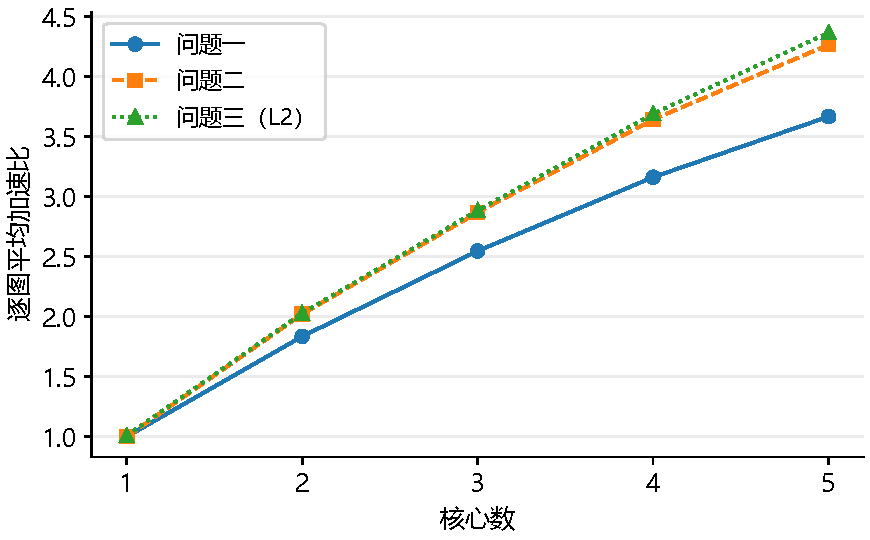
\includegraphics[width=0.85\linewidth,height=0.70\textheight,keepaspectratio]{../图表/runs/20260926-A-q123-complete-delivery/speedup.pdf}
\caption{三问逐图平均加速比（问题一取方案一；L2 单核沿用无 L2 参考）}\label{fig:q2-speed}\label{fig:q3-speed}
\end{figure}

\begin{figure}[!htbp]\centering
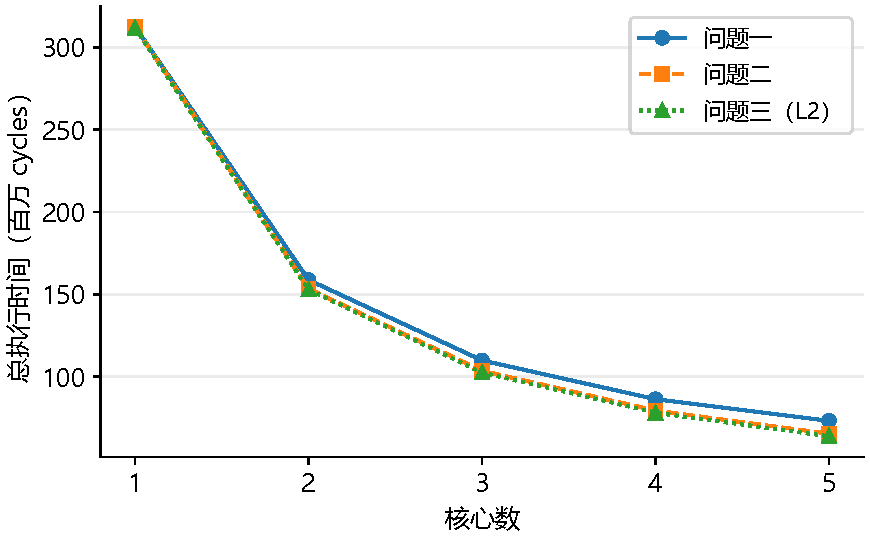
\includegraphics[width=0.85\linewidth,height=0.70\textheight,keepaspectratio]{../图表/runs/20260926-A-q123-complete-delivery/cycles.pdf}
\caption{三问百图总周期（问题一取方案一）}\label{fig:total-cycles}
\end{figure}
算法在每个核数独立搜索，增加核心数并不保证每个图都更快。全量结果证明与给定官方仿真一致，不构成全局最优证书或未见图泛化检验。
